\documentclass[12pt, a4paper]{article}

\usepackage{xcolor}	
 
%%%%%%%%%%%%%%%%%%%%%%%%%%%%%%%%%%%%%%%%%%%%%%%
% 				COLOURS
%%%%%%%%%%%%%%%%%%%%%%%%%%%%%%%%%%%%%%%%%%%%%%%

\definecolor{Red}{RGB}{128,0,0}
\definecolor{Blue}{RGB}{56,93,138}
\definecolor{Green}{RGB}{112,130,56}
\definecolor{Orange}{RGB}{255,133,50}
\definecolor{Magenta}{RGB}{139,0,139}
\definecolor{Brown}{RGB}{95,89,87}
\definecolor{Black}{RGB}{0,0,0}
\definecolor{White}{RGB}{255,255,255}
\definecolor{Gray}{RGB}{192,192,192}
%%%%%%%%%%%%%%%%%%%%%%%%%%%%%%%%%%%%%%%%%%%%%%%
% 				    MACROS
%%%%%%%%%%%%%%%%%%%%%%%%%%%%%%%%%%%%%%%%%%%%%%%

% Parentheses
\newcommand{\plbr}[1]	            { \left( #1 \right) }
\newcommand{\sqbr}[1]	            { \left[ #1 \right] }
\newcommand{\lcubr}[1]	            { \left\{ #1 \right.}

% Vectors and matrices
\newcommand{\cvvect}[1]	            { \begin{array}{c} #1 \end{array} }
\newcommand{\hvect}[2]	            { \begin{array}{ #1 } #2 \end{array} }
\newcommand{\matr}[2]	            { \begin{array}{ #1 } #2 \end{array} }

% Units
\newcommand{\unit}[1]				{ {\; \mathrm {#1}} }
\newcommand{\point}[1]				{ \mathsf{ #1 } }

% General notation
\newcommand{\ctime}					{ t }
\newcommand{\stepSize}				{ {\textrm d} \ctime}
\newcommand{\step}                  { k }


% Co-simulation notation - fundamentals
\newcommand{\state}					{ \mathbf{ x } }
\newcommand{\derivative}            { \dot{\state} }
\newcommand{\inputMod}				{ u }
\newcommand{\outputMod}				{ y }
\newcommand{\forceMod}				{ f }
\newcommand{\inputs}				{ { \inputMod} }
\newcommand{\outputs}				{ { \outputMod} }
\newcommand{\force}					{ { \forceMod} }
\newcommand{\microstep}				{ h }
\newcommand{\communicationstep}		{ H }
\newcommand{\forceCorr}             { \tilde{\forceMod} }
\newcommand{\nextApproxInput}       { \tilde{\inputs} }

% Subscripts and superscripts
\newcommand{\trans}   				{ ^{\textrm T}}
\newcommand{\inv}   				{ ^{\textrm -1}}
\newcommand{\extr}   				{ ^{\textrm *}}


% Schemes
\newcommand{\angles}				{ \theta }
\newcommand{\cyldisplacement}		{ s_c }
\newcommand{\cylvelocity}			{ \dot{s}_c }
\newcommand{\discharge}				{ c_d }
\newcommand{\density}     			{ \rho }
\newcommand{\bulkMod}				{ \beta }
\newcommand{\outputValve}			{ a_o }
\newcommand{\inputValve}			{ a_i }
\newcommand{\compressibilityA}		{ a }
\newcommand{\compressibilityB}		{ b }
\newcommand{\spool}					{ \gamma }
\newcommand{\cyldisplacementIni}	{ s_c^0 }
\newcommand{\amplitude}				{ A }
\newcommand{\angular}				{ \omega }
\newcommand{\pressure}				{ p }
\newcommand{\power}                 { P }
\newcommand{\Residualpower}         { \delta \power }
\newcommand{\stiffness}				{ \kappa }
\newcommand{\damping}				{ c }
\newcommand{\mass}					{ m }
\newcommand{\length}				{ l }
\newcommand{\displacement}			{ \eta }
\newcommand{\velocity}				{ \dot{\eta} }
\newcommand{\acceleration}			{ \ddot{\eta} }
\newcommand{\piston}				{ a_p }
\newcommand{\matLO}					{ \bm{\Theta} }


% State-space - fundamentals
\newcommand{\stateMatrix}			{ \mathbf{A} }
\newcommand{\inputMatrix}			{ \mathbf{B} }
\newcommand{\outputMatrix}			{ \mathbf{C} }
\newcommand{\feedthrough}			{ \mathbf{D} }

% Matrices
\newcommand{\identity}				{ \mathbf{I} }
\newcommand{\zero}					{ \mathbf{0} }

% Estimadores
\newcommand{\estimation}            { \mathbf{X} }
\newcommand{\estimated}             { Y }
\newcommand{\coefficient}           { \alpha}
\newcommand{\coefficients}          { \bm{\coefficient}}

\usepackage{tikz}
\usepackage{amsmath}

\usetikzlibrary{external}
\tikzexternalize

\begin{document}

\begin{figure}[ht!]\centering
	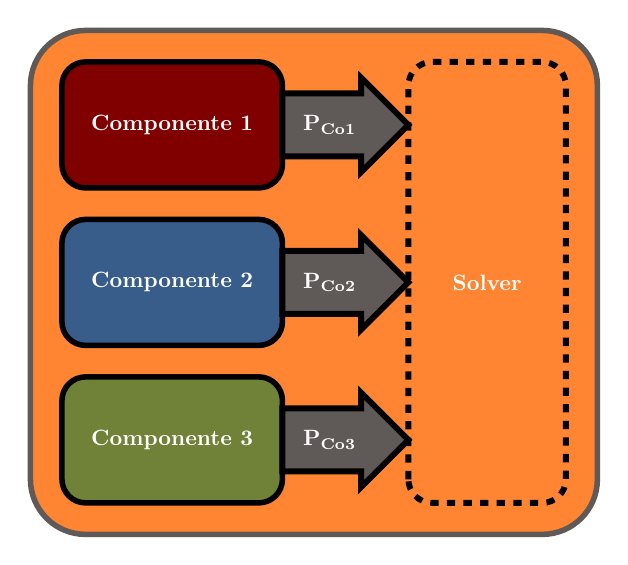
\begin{tikzpicture}[scale=0.8, transform shape] 
		
		% Rectangle
		\filldraw [fill=Orange, draw=Brown, rounded corners=0.7cm, line width=2pt] (-4,0) rectangle (5,8);	
		\filldraw [fill=Red, draw=Black, rounded corners=0.3cm, line width=2pt] (-3.5,7.5) rectangle (0,5.5);
		\filldraw [fill=Green, draw=Black, rounded corners=0.3cm, line width=2pt] (-3.5,2.5) rectangle (0,0.5);
		\filldraw [fill=Blue, draw=Black, rounded corners=0.3cm, line width=2pt] (-3.5,5) rectangle (0,3);
		\draw [draw=Black, dashed, rounded corners=0.3cm,line width=0.75mm] (2,0.5) -- (2,7.5) -- (4.5,7.5) -- (4.5,0.5)-- cycle;	
		
		% Flows
		\filldraw [fill=Brown, draw=Black, line width=0.75mm] (0,1) -- (0,2) -- (1.25,2) -- (1.25,2.25) -- (2,1.5) -- (1.25,0.75) -- (1.25,1) -- cycle;
		
		\filldraw [fill=Brown, draw=Black, line width=0.75mm] (0,3.5) -- (0,4.5) -- (1.25,4.5) -- (1.25,4.75) -- (2,4) -- (1.25,3.25) -- (1.25,3.5) -- cycle;
		
		\filldraw [fill=Brown, draw=Black, line width=0.75mm] (0,6) -- (0,7) -- (1.25,7) -- (1.25,7.25) -- (2,6.5) -- (1.25,5.75) -- (1.25,6) -- cycle;
		
		% Text		
		\node[align=center, color = White] at (-17.5mm, 65mm) {\textbf{Componente 1}};
		\node[align=center, color = White] at (-17.5mm, 40mm) {\textbf{Componente 2}};
		\node[align=center, color = White] at (-17.5mm, 15mm) {\textbf{Componente 3}};
		
		\node[align=center, color = White] 			at (7.5mm, 65mm) {$\mathbf{\power_{Co1}}$};
		\node[align=center, color = White] 			at (7.5mm, 40mm) {$\mathbf{\power_{Co2}}$};
		\node[align=center, color = White] 			at (7.5mm, 15mm) {$\mathbf{\power_{Co3}}$};
		
		\node[align=center, color = White] at (32.5mm, 40mm) {\textbf{Solver}};
		
	\end{tikzpicture}
\end{figure}

\begin{figure}[ht!]\centering
	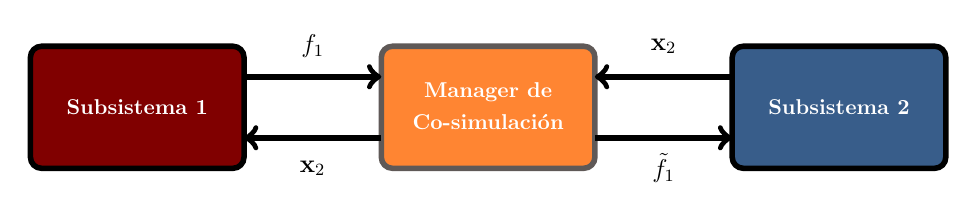
\begin{tikzpicture}[scale=0.775, transform shape] 
		
		% Rectangle
		\filldraw [fill=Red, draw=Black, line width=2pt, rounded corners] (-7.5,0) rectangle (-4,2);
		\filldraw [fill=Orange, draw=Brown, line width=2pt, rounded corners] (-1.75,0) rectangle (1.75,2);
		\filldraw [fill=Blue, draw=Black, line width=2pt, rounded corners] (4,0) rectangle (7.5,2);
		
		
		% Text
		\node[align=center, color = White] 			at (0mm, 12.5mm) {\textbf{Manager de}};
		\node[align=center, color = White] 			at (0mm, 7.5mm) {\textbf{Co-simulación}};
		
		\node[align=center, color = White] 			at (-57.5mm, 10mm) {\textbf{Subsistema 1}};
		\node[align=center, color = White] 			at (57.5mm, 10mm) {\textbf{Subsistema 2}};
		
		% Lines
		\draw[->, line width=0.75mm] (-4,1.5) -- (-1.75,1.5);
		\draw[<-, line width=0.75mm] (1.75,1.5) -- (4,1.5);
		\draw[->, line width=0.75mm] (1.75,0.5) -- (4,0.5);
		\draw[<-, line width=0.75mm] (-4,0.5) -- (-1.75,0.5);
		
		% Variables
		\node[align=center, color = Black, font=\large] 			at (28.75mm, 0mm) {$\forceCorr_1$};
		\node[align=center, color = Black, font=\large] 			at (-28.75mm, 20mm) {$\forceMod_1$};
		\node[align=center, color = Black, font=\large] 			at (28.75mm, 20mm) {$\state_2$};
		\node[align=center, color = Black, font=\large] 			at (-28.75mm, 0mm) {$\state_2$};
		
	\end{tikzpicture}
\end{figure}

\begin{figure}[ht!]\centering
	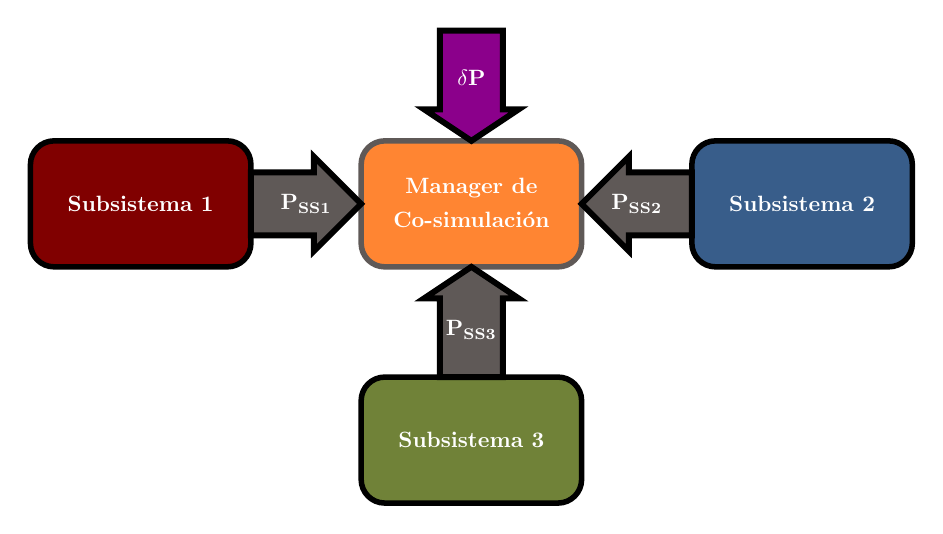
\begin{tikzpicture}[scale=0.8, transform shape] 
		
		% Rectangle
		\filldraw [fill=Orange, draw=Brown, rounded corners=0.3cm, line width=2pt] (-1.75,0) rectangle (1.75,2);	
		\filldraw [fill=Blue, draw=Black, rounded corners=0.3cm, line width=2pt] (3.5,0) rectangle (7,2);
		\filldraw [fill=Red, draw=Black, rounded corners=0.3cm, line width=2pt] (-3.5,0) rectangle (-7,2);
		\filldraw [fill=Green, draw=Black, rounded corners=0.3cm, line width=2pt] (-1.75,-3.75) rectangle (1.75,-1.75);
		
		% Text
		\node[align=center, color = White] at (0mm, 12.5mm) {\textbf{Manager de}};
		\node[align=center, color = White] at (0mm, 7.5mm) {\textbf{Co-simulación}};
		
		\node[align=center, color = White] at (-52.5mm, 10mm) {\textbf{Subsistema 1}};
		
		\node[align=center, color = White] at (52.5mm, 10mm) {\textbf{Subsistema 2}};
		
		\node[align=center, color = White] at (0mm, -27.5mm) {\textbf{Subsistema 3}};
		
		% Flows
		\filldraw [fill=Brown, draw=Black, line width=0.75mm] (-3.5,0.5) -- (-3.5,1.5) -- (-2.5,1.5) -- (-2.5,1.75) -- (-1.75,1) -- (-2.5,0.25) -- (-2.5,0.5) -- cycle;
		
		\filldraw [fill=Brown, draw=Black, line width=0.75mm] (3.5,0.5) -- (3.5,1.5) -- (2.5,1.5) -- (2.5,1.75) -- (1.75,1) -- (2.5,0.25) -- (2.5,0.5) -- cycle;
		
		\filldraw [fill=Brown, draw=Black, line width=0.75mm] (0.5,-1.75) -- (-0.5,-1.75) -- (-0.5,-0.5) -- (-0.75,-0.5) -- (0,0) -- (0.75,-0.5) -- (0.5,-0.5) -- cycle;
		
		\filldraw [fill=Magenta, draw=Black, line width=0.75mm] (0.5,3.75) -- (-0.5,3.75) -- (-0.5,2.5) -- (-0.75,2.5) -- (0,2) -- (0.75,2.5) -- (0.5,2.5) -- cycle;
		
		% Exchanged
		\node[align=center, color = White] 			at (-26.25mm, 10mm) {$\mathbf{\power_{SS1}}$};
		\node[align=center, color = White] 			at (26.25mm, 10mm) {$\mathbf{\power_{SS2}}$};
		
		\node[align=center, color = White] 			at (0mm, -10mm) {$\mathbf{\power_{SS3}}$};
		
		\node[align=center, color = White] 			at (0mm, 30mm) {$\mathbf{\Residualpower}$};
		
		
	\end{tikzpicture}
\end{figure}


\begin{figure}[ht!]\centering
	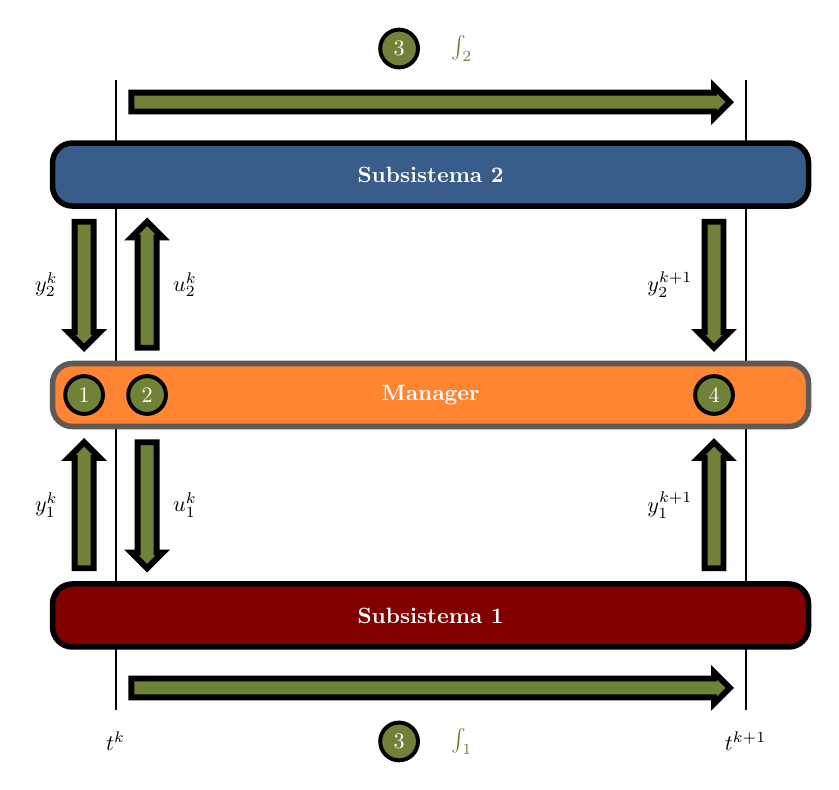
\begin{tikzpicture}[scale=0.8, transform shape] 
		
		% Steps
		\draw[-, draw=Black, line width=0.25mm] (-5,5) -- (-5,-5);
		\draw[-, draw=Black, line width=0.25mm] (5,5) -- (5,-5);
		
		% Blocks
		\filldraw [fill=Orange, draw=Brown, rounded corners=0.25cm, line width=2pt] (-6,-0.5) rectangle (6,0.5);
		\filldraw [fill=Blue, draw=Black, rounded corners=0.25cm, line width=2pt] (-6,3) rectangle (6,4);
		\filldraw [fill=Red, draw=Black, rounded corners=0.25cm, line width=2pt] (-6,-4) rectangle (6,-3);
		
		% Names
		\node[align=center, color = White] at (0mm, 0mm) {\textbf{Manager}};
		\node[align=center, color = White] at (0mm, -35mm) {\textbf{Subsistema 1}};
		\node[align=center, color = White] at (0mm, 35mm) {\textbf{Subsistema 2}};
		
		% Exchange
		\node[align=center, color = Black] at (-61mm, 17.5mm) {$\outputs_2^{\step}$};
		\node[align=center, color = Black] at (-61mm, -17.5mm) {$\outputs_1^{\step}$};
		
		\node[align=center, color = Black] at (-39mm, 17.5mm) {$\inputs_2^{\step}$};
		\node[align=center, color = Black] at (-39mm, -17.5mm) {$\inputs_1^{\step}$};
		
		\node[align=center, color = Black] at (38mm, 17.5mm) {$\outputs_2^{\step + 1}$};
		\node[align=center, color = Black] at (38mm, -17.5mm) {$\outputs_1^{\step + 1}$};
		
		% Communication
		\node[align=center, color = Black] at (-50mm, -55mm) {$\ctime^{\step}$};
		\node[align=center, color = Black] at (50mm, -55mm) {$\ctime^{\step + 1}$};
		
		% Flow
		\filldraw [fill=Green, draw=Black, line width=0.75mm] (-4.75,4.5) -- (4.5,4.5) -- (4.5,4.4) -- (4.75,4.65) -- (4.5,4.9) -- (4.5,4.8) -- (-4.75,4.8) -- cycle;
		
		\filldraw [fill=Green, draw=Black, line width=0.75mm] (-4.75,-4.5) -- (4.5,-4.5) -- (4.5,-4.4) -- (4.75,-4.65) -- (4.5,-4.9) -- (4.5,-4.8) -- (-4.75,-4.8) -- cycle;
		
		\filldraw [fill=Green, draw=Black, line width=0.75mm] (-4.65,0.75) -- (-4.35,0.75) -- (-4.35,2.5) -- (-4.25,2.5) -- (-4.5,2.75) -- (-4.75,2.5) -- (-4.65,2.5) -- cycle;
		
		\filldraw [fill=Green, draw=Black, line width=0.75mm] (-4.65,-0.75) -- (-4.35,-0.75) -- (-4.35,-2.5) -- (-4.25,-2.5) -- (-4.5,-2.75) -- (-4.75,-2.5) -- (-4.65,-2.5) -- cycle;
		
		\filldraw [fill=Green, draw=Black, line width=0.75mm] (-5.65,2.75) -- (-5.65,1) -- (-5.75,1) -- (-5.5,0.75) -- (-5.25,1) -- (-5.35,1) -- (-5.35,2.75) -- cycle;
		
		\filldraw [fill=Green, draw=Black, line width=0.75mm] (-5.65,-2.75) -- (-5.65,-1) -- (-5.75,-1) -- (-5.5,-0.75) -- (-5.25,-1) -- (-5.35,-1) -- (-5.35,-2.75) -- cycle;
		
		\filldraw [fill=Green, draw=Black, line width=0.75mm] (4.35,2.75) -- (4.35,1) -- (4.25,1) -- (4.5,0.75) -- (4.75,1) -- (4.65,1) -- (4.65,2.75) -- cycle;
		
		\filldraw [fill=Green, draw=Black, line width=0.75mm] (4.35,-2.75) -- (4.35,-1) -- (4.25,-1) -- (4.5,-0.75) -- (4.75,-1) -- (4.65,-1) -- (4.65,-2.75) -- cycle;
		
		% Order		
		\draw[fill=Green, draw=Black, line width=0.5mm] (-4.5,0) circle (3mm);
		\draw[fill=Green, draw=Black, line width=0.5mm] (-5.5,0) circle (3mm);
		\draw[fill=Green, draw=Black, line width=0.5mm] (4.5,0) circle (3mm);
		\draw[fill=Green, draw=Black, line width=0.5mm] (-0.5,5.5) circle (3mm);
		\draw[fill=Green, draw=Black, line width=0.5mm] (-0.5,-5.5) circle (3mm);
		
		\node[align=center, color = White] at (-55mm, 0mm) {$1$};
		\node[align=center, color = White] at (-45mm, 0mm) {$2$};
		\node[align=center, color = White] at (45mm, 0mm) {$4$};
		\node[align=center, color = White] at (-5mm,-55mm) {$3$};
		\node[align=center, color = White] at (-5mm, 55mm) {$3$};
		\node[align=center, color = Green] at (5mm,-55mm) {$\int_1$};
		\node[align=center, color = Green] at (5mm, 55mm) {$\int_2$};
		
	\end{tikzpicture} 
\end{figure}


\begin{figure}[ht!]\centering
	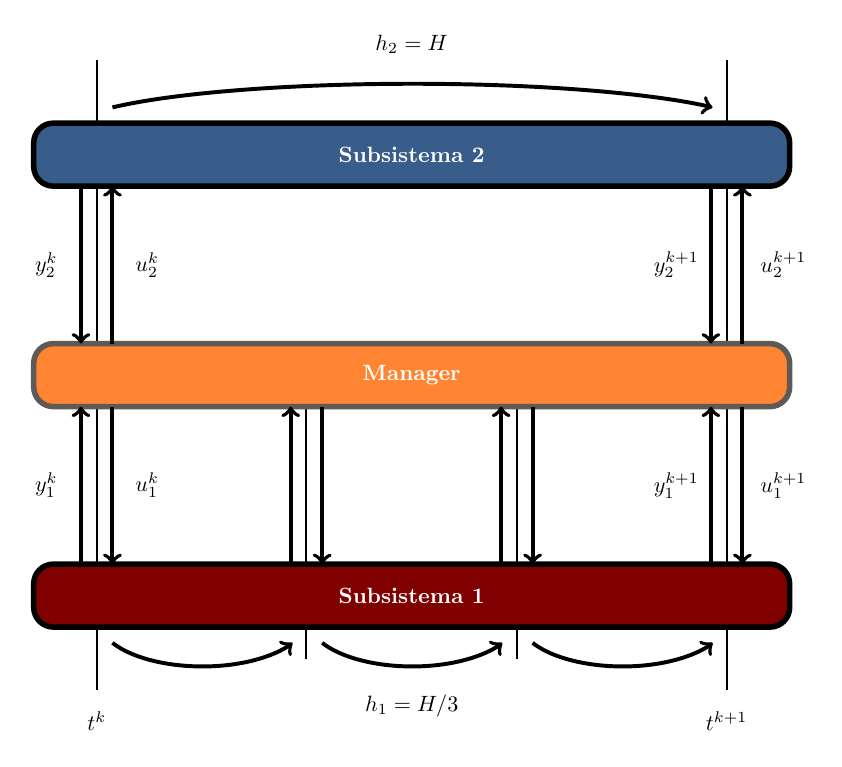
\begin{tikzpicture}[scale=0.8, transform shape] 
		
		% Steps
		\draw[-, draw=Black, line width=0.25mm] (-5,5) -- (-5,-5);
		\draw[-, draw=Black, line width=0.25mm] (5,5) -- (5,-5);
		\draw[-, draw=Black, line width=0.25mm] (-1.67,-4.5) -- (-1.67,-0.5);
		\draw[-, draw=Black, line width=0.25mm] (1.67,-4.5) -- (1.67,-0.5);
		
		% Blocks
		\filldraw [fill=Orange, draw=Brown, rounded corners=0.25cm, line width=2pt] (-6,-0.5) rectangle (6,0.5);
		\filldraw [fill=Blue, draw=Black, rounded corners=0.25cm, line width=2pt] (-6,3) rectangle (6,4);
		\filldraw [fill=Red, draw=Black, rounded corners=0.25cm, line width=2pt] (-6,-4) rectangle (6,-3);
		
		% Names
		\node[align=center, color = White] at (0mm, 0mm) {\textbf{Manager}};
		\node[align=center, color = White] at (0mm, -35mm) {\textbf{Subsistema 1}};
		\node[align=center, color = White] at (0mm, 35mm) {\textbf{Subsistema 2}};
		
		% Exchange
		\draw[->, draw=Black, line width=0.5mm] (-5.25,3) -- (-5.25,0.5);
		\draw[<-, draw=Black, line width=0.5mm] (-4.75,3) -- (-4.75,0.5);
		
		\draw[->, draw=Black, line width=0.5mm] (-5.25,-3) -- (-5.25,-0.5);
		\draw[<-, draw=Black, line width=0.5mm] (-4.75,-3) -- (-4.75,-0.5);
		
		\draw[<-, draw=Black, line width=0.5mm] (5.25,3) -- (5.25,0.5);
		\draw[->, draw=Black, line width=0.5mm] (4.75,3) -- (4.75,0.5);
		
		\draw[<-, draw=Black, line width=0.5mm] (5.25,-3) -- (5.25,-0.5);
		\draw[->, draw=Black, line width=0.5mm] (4.75,-3) -- (4.75,-0.5);
		
		\draw[->, draw=Black, line width=0.5mm] (-1.92,-3) -- (-1.92,-0.5);
		\draw[<-, draw=Black, line width=0.5mm] (-1.42,-3) -- (-1.42,-0.5);
		
		\draw[<-, draw=Black, line width=0.5mm] (1.92,-3) -- (1.92,-0.5);
		\draw[->, draw=Black, line width=0.5mm] (1.42,-3) -- (1.42,-0.5);
		
		% Variables
		\node[align=center, color = Black] at (-42mm, 17.5mm) {$\inputs_2^{\step}$};
		\node[align=center, color = Black] at (-58mm, 17.5mm) {$\outputs_2^{\step}$};
		
		\node[align=center, color = Black] at (-42mm, -17.5mm) {$\inputs_1^{\step}$};
		\node[align=center, color = Black] at (-58mm, -17.5mm) {$\outputs_1^{\step}$};
		
		\node[align=center, color = Black] at (59mm, 17.5mm) {$\inputs_2^{\step + 1}$};
		\node[align=center, color = Black] at (42mm, 17.5mm) {$\outputs_2^{\step + 1}$};
		
		\node[align=center, color = Black] at (59mm, -17.5mm) {$\inputs_1^{\step + 1}$};
		\node[align=center, color = Black] at (42mm, -17.5mm) {$\outputs_1^{\step + 1}$};
		
		%\node[align=center, color = Black] at (-27mm, -25mm) {$\outputs\first_{\currentTime + \microstep\firstSub}$};
		%\node[align=center, color = Black] at (-5mm, -10mm) {$\inputs\first_{\currentTime + \microstep\firstSub}$};
		
		%\node[align=center, color = Black] at (5mm, -25mm) {$\outputs\first_{\currentTime + 2\microstep\firstSub}$};
		%\node[align=center, color = Black] at (29mm, -10mm) {$\inputs\first_{\currentTime + 2\microstep\firstSub}$};
		
		
		% Communication
		\draw[->, draw=Black, line width=0.5mm] (-4.75,4.25) arc[start angle = 30, end angle = 150, x radius = -5.5, y radius = 0.75];
		
		\draw[->, draw=Black, line width=0.5mm] (-4.75,-4.25) arc[start angle = 30, end angle = 150, x radius = -1.65, y radius = -0.75];
		\draw[->, draw=Black, line width=0.5mm] (-1.42,-4.25) arc[start angle = 30, end angle = 150, x radius = -1.65, y radius = -0.75];
		\draw[->, draw=Black, line width=0.5mm] (1.92,-4.25) arc[start angle = 30, end angle = 150, x radius = -1.65, y radius = -0.75];
		
		\node[align=center, color = Black] at (0mm, -52.5mm) {$\microstep_1 = \communicationstep / 3$};
		\node[align=center, color = Black] at (0mm, 52.5mm) {$\microstep_2 = \communicationstep$};
		
		\node[align=center, color = Black] at (-50mm, -55mm) {$\ctime^{\step}$};
		\node[align=center, color = Black] at (50mm, -55mm) {$\ctime^{\step + 1}$};
		
		
	\end{tikzpicture} 
\end{figure}


\begin{figure}[ht!]\centering
	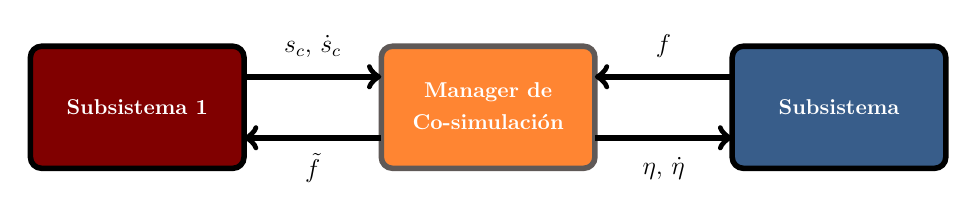
\begin{tikzpicture}[scale=0.775, transform shape] 
		
		% Rectangle
		\filldraw [fill=Red, draw=Black, line width=2pt, rounded corners] (-7.5,0) rectangle (-4,2);
		\filldraw [fill=Orange, draw=Brown, line width=2pt, rounded corners] (-1.75,0) rectangle (1.75,2);
		\filldraw [fill=Blue, draw=Black, line width=2pt, rounded corners] (4,0) rectangle (7.5,2);
		
		
		% Text
		\node[align=center, color = White] 			at (0mm, 12.5mm) {\textbf{Manager de}};
		\node[align=center, color = White] 			at (0mm, 7.5mm) {\textbf{Co-simulación}};
		
		\node[align=center, color = White] 			at (-57.5mm, 10mm) {\textbf{Subsistema 1}};
		\node[align=center, color = White] 			at (57.5mm, 10mm) {\textbf{Subsistema}};
		
		% Lines
		\draw[->, line width=0.75mm] (-4,1.5) -- (-1.75,1.5);
		\draw[<-, line width=0.75mm] (1.75,1.5) -- (4,1.5);
		\draw[->, line width=0.75mm] (1.75,0.5) -- (4,0.5);
		\draw[<-, line width=0.75mm] (-4,0.5) -- (-1.75,0.5);
		
		% Variables
		\node[align=center, color = Black, font=\large] 			at (28.75mm, 0mm) {$\displacement$, $\velocity$};
		\node[align=center, color = Black, font=\large] 			at (-28.75mm, 20mm) {$\cyldisplacement$, $\cylvelocity$};
		\node[align=center, color = Black, font=\large] 			at (28.75mm, 20mm) {$\forceMod$};
		\node[align=center, color = Black, font=\large] 			at (-28.75mm, 0mm) {$\forceCorr$};
		
	\end{tikzpicture}
\end{figure}


\begin{figure}[ht!]\centering
	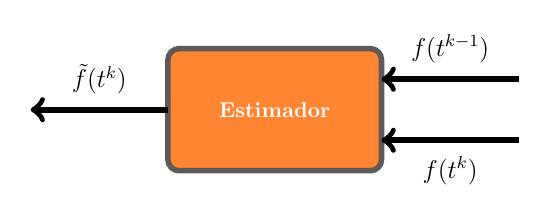
\begin{tikzpicture}[scale=0.775, transform shape] 
		
		% Rectangle
		\filldraw [fill=Orange, draw=Brown, line width=2pt, rounded corners] (-1.75,0) rectangle (1.75,2);
		
		
		% Text
		\node[align=center, color = White] 			at (0mm, 10mm) {\textbf{Estimador}};


		% Lines
		\draw[<-, line width=0.75mm] (-4,1.0) -- (-1.75,1.0);
		\draw[<-, line width=0.75mm] (1.75,1.5) -- (4,1.5);
		\draw[<-, line width=0.75mm] (1.75,0.5) -- (4,0.5);
		
		% Variables
		\node[align=center, color = Black, font=\large] 			at (28.75mm, 0mm) {$\forceMod (\ctime^{\step})$};
		\node[align=center, color = Black, font=\large] 			at (28.75mm, 20mm) {$\forceMod (\ctime^{\step - 1})$};
		\node[align=center, color = Black, font=\large] 			at (-28.75mm, 15mm) {$\forceCorr (\ctime^{\step})$};
		
	\end{tikzpicture}
\end{figure}

\end{document}